\documentclass[class=article, crop=false]{standalone}
\usepackage[subpreambles=true]{standalone}
\usepackage{import}
\usepackage{preamble}
\usepackage{pdfpages}
\usepackage{pgfplots}
\usepackage{pgfplotstable}
\begin{document}
\pgfplotsset{
%        compat=newest,  % <-- does not work; don't know why
        compat=1.13,     % <-- works as expected
    }
  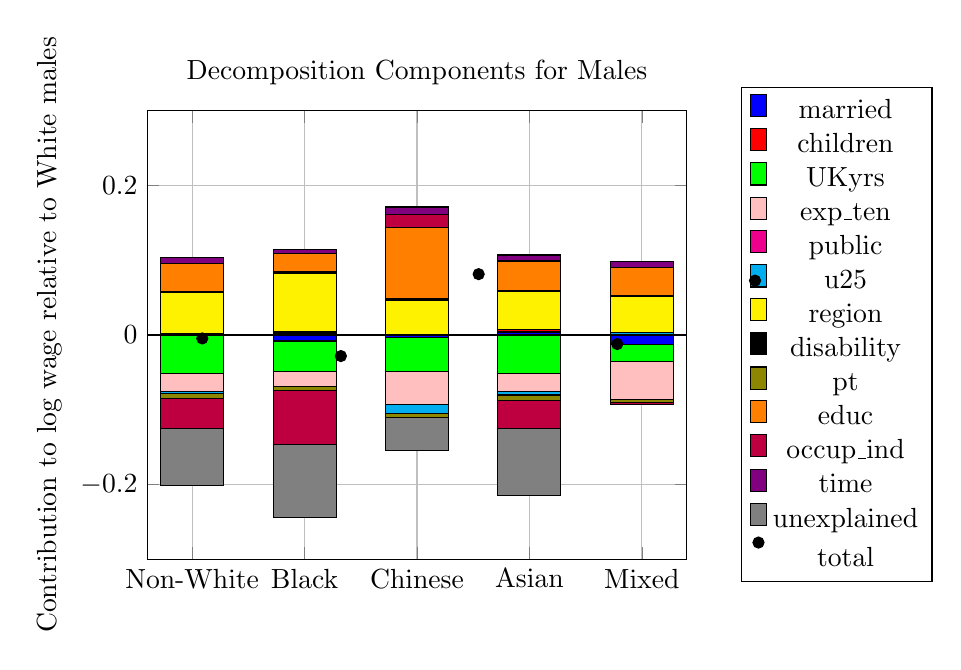
\begin{tikzpicture}
  %\node [align=center, font=\small, rotate=45,text width=2.15cm, inner sep=0.25cm] at (1, 1) {\textsc{year 1}};
%   \addplot[only marks,mark=*,mark size=3pt,black,
%          nodes near coords = \rotatebox{90}{{\pgfmathprintnumber[fixed zerofill,
%                                     precision=2]{\pgfplotspointmeta}}},
%         nodes near coords align={vertical},
%         point meta=y,
%         every node near coord/.append style={font=\small, yshift=0.25mm},
%         ]  coordinates {
%     (1,0.1) (2,-0.1) (3,1)
% };
%\fill [fill=red, fill opacity=0.1] (0,0) node[left]{} -- (0,3.5) node[below left] {} -- (8.4,3.5) node[below left] {} -- (8.4,0) node[below left] {};
%\fill [fill=green, fill opacity=0.1] (0,3.5) node[left]{} -- (0,7.05) node[below left] {} -- (8.4,7.05) node[below left] {} -- (8.4,3.5) node[below left] {};
  \begin{axis}[
    title={Decomposition Components for Males},
    ybar stacked,
    ymax=0.3,
    ymin=-0.3,
    ylabel=Contribution to log wage relative to White males,
    ymajorgrids = true,
    xmajorgrids = true,
    bar width=8mm,
    %xtick={1,2,3,4,5},
    %xticklabels={White, Black, Chinese, Asian, Mixed}
    symbolic x coords={Non-White, Black, Chinese, Asian, Mixed},
    xtick=data,
    nodes near coords align={anchor=north},%Move values in bar
    every node near coord/.style={},
    legend style={at={(1.1,0.5)},anchor=west}
  ]
%married
\addplot [fill=blue] coordinates {({Non-White},-0.0007476)({Black},-0.0081719)({Chinese},-0.0039328)({Asian},0.0039439)({Mixed},-0.0123207)};
%children
\addplot [fill=red] coordinates {({Non-White},0.0023548)({Black},0.0026034)({Chinese},0.0001847)({Asian},0.0033247)({Mixed},0.00019)};
%UKyrs
\addplot [fill=green] coordinates {({Non-White},-0.050569)({Black},-0.0410711)({Chinese},-0.0452143)({Asian},-0.0512385)({Mixed},-0.0235874)};
%exp_ten
\addplot [fill=pink] coordinates {({Non-White},-0.0250038)({Black},-0.0197287)({Chinese},-0.0435713)({Asian},-0.0248561)({Mixed},-0.050915)};
%public
\addplot [fill=magenta] coordinates {({Non-White},-0.0000000612)({Black},0.0000988)({Chinese},0.0000228)({Asian},-0.0001474)({Mixed},0.0000252)};
%u25
\addplot [fill=cyan] coordinates {({Non-White},-0.0026008)({Black},0.0014516)({Chinese},-0.0127419)({Asian},-0.004224)({Mixed},0.0031096)};
%region
\addplot [fill=yellow] coordinates {({Non-White},0.0544848)({Black},0.0782871)({Chinese},0.0459306)({Asian},0.0512847)({Mixed},0.0488203)};
%disability
\addplot [fill=black] coordinates {({Non-White},0.0010427)({Black},0.0017822)({Chinese},0.002456)({Asian},0.0007188)({Mixed},0.0003888)};
%pt
\addplot [fill=olive] coordinates {({Non-White},-0.0060493)({Black},-0.0055884)({Chinese},-0.0054992)({Asian},-0.0067801)({Mixed},-0.0033902)};
%educ
\addplot [fill=orange] coordinates {({Non-White},0.0377985)({Black},0.0248366)({Chinese},0.0945977)({Asian},0.0396925)({Mixed},0.0371787)};
%occup_ind
\addplot [fill=purple] coordinates {({Non-White},-0.0407851)({Black},-0.0721109)({Chinese},0.0184845)({Asian},-0.038575)({Mixed},-0.0028553)};
%time
\addplot [fill=violet] coordinates {({Non-White},0.0075861)({Black},0.0057739)({Chinese},0.0095596)({Asian},0.0079793)({Mixed},0.0086406)};
%unexplained
\addplot [fill=gray] coordinates
{({Non-White},-0.0758006)({Black},-0.0979634)({Chinese},-0.0435532)({Asian},-0.0894198)({Mixed},-0.0001854)};

\addplot [only marks,mark=*,mark size=2pt,black,
         nodes near coords = \rotatebox{90}{{\pgfmathprintnumber[fixed zerofill,
                                    precision=2]{\pgfplotspointmeta}}},
        nodes near coords align={vertical},
        point meta=y,
        every node near coord/.append style={font=\small, yshift=0.25mm},] coordinates {({Mixed},-1)};
%\begin{comment}
%\end{comment}
%\filldraw[black] (0,0) circle (2pt) node[anchor=west] {Intersection point};
  \legend{married, children, UKyrs, exp\_ten, public, u25, region, disability, pt, educ, occup\_ind, time, unexplained, total}
  \end{axis}
  
  \begin{axis}[
    nodes near coords align={anchor=north},%Move values in bar
    every node near coord/.style={},
    xtick=data,
    ymax=0.3,
    ymin=-0.3,
    xmax=0,
    xmin=5,
]
\pgfplotsset{ticks=none}
\addplot[only marks,mark=*,mark size=3pt,black,
         nodes near coords = \rotatebox{90}{{\pgfmathprintnumber[fixed zerofill,
                                    precision=2]{\pgfplotspointmeta}}},
        nodes near coords align={vertical},
        point meta=y,
        every node near coord/.append style={font=\small, yshift=0.25mm},
        ]  coordinates {
    (1,0.1) (2,-0.1) (3,1)
};
\addplot[color=black,thick] coordinates {(-6,0) (6,0)};
\end{axis}
\filldraw[black] (0.7,2.80214597) circle (2pt) node[anchor=west] {};
\filldraw[black] (2.46,2.57841432) circle (2pt) node[anchor=west] {};
\filldraw[black] (4.21,3.61873614) circle (2pt) node[anchor=west] {};
\filldraw[black] (5.97,2.73109201) circle (2pt) node[anchor=west] {};
\filldraw[black] (7.72,3.5362029) circle (2pt) node[anchor=west] {};
  \end{tikzpicture}
\end{document}